% ============================================================
%  Chapter 7 – Methods and Algorithms of the
%               Fixed-Point Thermal Control Benchmark
% ============================================================
% Intended for inclusion in a larger dissertation via \include{}
% or \input{}.  Requires the following packages in the preamble:
%   \usepackage{amsmath, amssymb, booktabs, array, longtable,
%               xcolor, graphicx, hyperref, caption, geometry}
% ============================================================

\chapter{Methods and Algorithms of the Fixed-Point Thermal Control Benchmark}
\label{chap:fpga_benchmark}

% ============================================================
\section{Introduction}
\label{sec:bench_intro}
% ============================================================

The preceding chapter described experiments conducted with the
Free-Form Spatial Reference (FFSR) benchmark to evaluate FPGA behaviour
under irradiation.  The present chapter introduces a complementary
benchmark designed for the same class of irradiation campaign, but with
a richer computational workload and built-in self-comparison capability.
Whereas the FFSR design exercised basic reconfiguration and readback
paths, the fixed-point thermal control benchmark couples closed-loop
feedback control, emulated physical plant dynamics, nonlinear actuator
mapping, and dual-modular redundancy (DMR) within a single synthesizable
Verilog design.  Because the two benchmarks share the same neutron
irradiation facility and beam configuration, the experimental
infrastructure described in Chapter~\ref{chap:ffsr} applies directly
here, and the present chapter focuses exclusively on the design methods,
algorithms, and implementation choices that distinguish this benchmark.

The benchmark is implemented entirely in synthesizable, fixed-point
Verilog and is intended to operate continuously during an irradiation
session, producing a 100\,Hz serial telemetry stream that records the
internal state of the control loop.  Any radiation-induced perturbation
that alters arithmetic results, corrupts stored state, or disrupts the
routing of signals within the FPGA is therefore observable in real time
through the telemetry output or, for subtle divergences, through the
pipelined mismatch flag generated by the DMR wrapper.  This combination
of control significance and fault-detection capability makes the
benchmark especially well suited to in-situ FPGA irradiation studies.

The remainder of this chapter is organized as follows.
Section~\ref{sec:bench_system} describes the top-level architecture and
design rationale.  Section~\ref{sec:bench_numrep} defines the
fixed-point number representation and sampling structure.
Sections~\ref{sec:bench_stimulus}--\ref{sec:bench_meas} present the
individual algorithmic subsystems in mathematical and implementation
detail.  Section~\ref{sec:bench_dmr} covers the redundancy, fault
detection, and telemetry mechanisms.
Section~\ref{sec:bench_timing} maps each RTL module to its mathematical
role.  Section~\ref{sec:bench_neutron} describes the neutron irradiation
experiment setup.  Section~\ref{sec:bench_observations} presents
comparative observations from two telemetry runs and discusses the
failure mechanism.  Section~\ref{sec:bench_relevance} discusses
relevance to the radiation-effects objectives of this dissertation, and
Section~\ref{sec:bench_summary} concludes with a chapter summary.

\begin{table}[h!]
  \centering
  \caption{Implementation snapshot---key parameters of the fixed-point
           thermal control benchmark as configured in the present
           irradiation experiments.}
  \label{tab:bench_snapshot}
  \renewcommand{\arraystretch}{1.25}
  \begin{tabular}{@{} p{4.5cm} p{9.5cm} @{}}
    \toprule
    \textbf{Parameter} & \textbf{Value / Description} \\
    \midrule
    Clock frequency          & 100\,MHz top-level system clock \\
    Control/plant sample rate & 1\,kHz global tick generated in the stimulus block \\
    Arithmetic format        & Predominantly signed Q1.15; Q1.30 internal
                               accumulation in the thermal plant \\
    Redundancy               & Two duplicated control-plant chains compared
                               inside the DMR wrapper with CSV-style UART telemetry \\
    Button control           & 20\,ms debounce; 3\,s hold to stop; short
                               press-and-release issues \texttt{restart\_pulse}
                               and resumes run mode \\
    UART output decimation   & \texttt{decim}~$= 10$, giving one CSV record
                               every 10\,ms (100\,Hz) while running \\
    DMR compare tolerance    & \texttt{dmr\_tol\_q15}~$= \texttt{0x0000}$
                               (exact comparison) \\
    \bottomrule
  \end{tabular}
\end{table}

% ============================================================
\section{System-Level Methodology}
\label{sec:bench_system}
% ============================================================

At the highest level, the benchmark is organized as a sampled-data loop
executed inside a single FPGA clock domain running at 100\,MHz.  A
one-cycle sample strobe at 1\,kHz acts as the logical update event for
the control algorithm, the plant emulation, and telemetry capture.  In
the current top-level implementation (\texttt{top\_pid\_thermal\_dmr.v}),
this strobe is generated in \texttt{u\_stim.v} and forwarded as the
global tick only while the run-enable signal is asserted, so the dynamic
state of the benchmark freezes when the experiment is stopped.  The
top-level integration additionally includes a dedicated power-on-reset
counter, button-driven run and restart control, a millisecond time base
that is reset by the restart pulse, the DMR-protected control-plant
core, and the UART output path.

The design is organized around five functional layers:
(1)~input stimulus generation,
(2)~the closed-loop control algorithm,
(3)~actuator and nonlinear valve mapping,
(4)~the two-node thermal plant and measurement model, and
(5)~redundancy and telemetry infrastructure.
Each layer is implemented in one or more dedicated RTL modules, and the
inter-module interfaces use fixed-point Q1.15 values throughout.

This methodology has several advantages for radiation-effects
experimentation.  First, the state evolution is deterministic and
repeatable, which allows observed anomalies to be attributed more
confidently to hardware perturbations rather than software timing
jitter.  Second, the use of bounded fixed-point states and saturating
arithmetic prevents uncontrolled numeric growth during upset conditions.
Third, the benchmark simultaneously exercises arithmetic pipelines,
state registers, lookup tables, comparators, counters, and serial
communication logic---all categories of FPGA resource that can respond
differently to configuration upsets or transient single-event effects.
Finally, the explicit run gating, exact DMR comparison, and
deterministic restart behaviour make it well suited to repeatable
irradiation campaigns where reproducible initial conditions are
important.

% ============================================================
\section{Numerical Representation and Sampling Structure}
\label{sec:bench_numrep}
% ============================================================

Nearly all signals in the design are encoded in signed Q1.15 format.
In this representation, a 16-bit signed integer $x_{\mathrm{q15}}$
represents the real quantity $x$ through the scaling relation

\begin{equation}
  x \;\approx\; \frac{x_{\mathrm{q15}}}{2^{15}} \,.
  \label{eq:q15_scaling}
\end{equation}

This choice provides compact arithmetic, deterministic synthesis, and
direct use of FPGA DSP-slice resources while maintaining sufficient
precision for the normalized thermal benchmark, where all physical
quantities are expressed as dimensionless fractions of their respective
full-scale values.

The reusable multiplier pipeline in \texttt{q15\_mul\_pipe.v} implements
rounded fixed-point multiplication.  For Q1.15 operands $a$ and $b$,
the full-precision product is formed in Q1.30, rounded by adding
one-half least-significant bit of the target scale, and then shifted
right by 15 bits:

\begin{equation}
  p_{\mathrm{q15}} \;=\; \mathrm{round}\!\left(
    \frac{a_{\mathrm{q15}} \cdot b_{\mathrm{q15}}}{2^{15}}
  \right) \,.
  \label{eq:q15_mul}
\end{equation}

Simple additions and subtractions that could exceed the numeric range
are performed with saturation rather than wraparound.  This is
especially important in a closed-loop design, because two's-complement
overflow produces nonphysical values that are indistinguishable in the
binary record from genuine radiation-induced upsets.  The thermal plant
goes one step further and stores its internal accumulator state in
signed Q1.30 format, thereby reducing deadband and truncation error in
the forward-Euler integration even though block inputs and outputs
remain Q1.15.

Sampling is derived from the 100\,MHz FPGA clock by a divider in
\texttt{u\_stim.v}.  One global tick is generated every 100,000
system-clock cycles, corresponding to a sample period $T_s = 1$\,ms.
Because \texttt{tick\_1k} is taken directly from the stimulus-valid
pulse, the controller, plant, DMR wrapper, and UART logger all advance
only when the benchmark is in run mode.  The control chain is pipelined
over several 100\,MHz cycles so that the algorithmic latency from tick
assertion to updated measured output is approximately 70\,ns---negligible
relative to the 1\,ms control period.

% ============================================================
\section{Input Stimulus and Run/Restart Control}
\label{sec:bench_stimulus}
% ============================================================

\subsection{Button-Controlled Run Logic}
\label{ssec:bench_button}

Human interaction with the benchmark during an irradiation session is
handled by \texttt{btn\_run\_ctrl.v}.  The pushbutton signal is
synchronized through a two-flip-flop chain to eliminate metastability,
then debounced by requiring a stable level for a programmable window of
20\,ms.  A short press-and-release sequence issues a one-cycle restart
pulse and enables run mode; a long press of at least 3\,s latches the
design into a stopped state.  This approach prevents mechanical bounce
from spuriously retriggering the experiment and provides an
operator-friendly means to restart the benchmark between irradiation
intervals without requiring FPGA reconfiguration.

\subsection{Stimulus Generator}
\label{ssec:bench_stim_gen}

The block \texttt{u\_stim.v} generates the closed-loop reference $r[k]$
and the disturbance (thermal power input) term $Q[k]$.  The pattern
repeats every 600\,s and is indexed by a millisecond counter
$t_{\mathrm{ms}}$ that wraps after 600\,000 updates.  The reference
target follows a piecewise-constant schedule, while the disturbance is
applied as a direct step profile:

\begin{equation}
  r_{\mathrm{tgt}}(t) \;=\;
  \begin{cases}
    0.55, & 0 \le t < 30\,\mathrm{s} \\
    0.60, & 30 \le t < 250\,\mathrm{s} \\
    0.57, & 250 \le t < 400\,\mathrm{s} \\
    0.61, & 400 \le t < 530\,\mathrm{s} \\
    0.55, & 530 \le t < 600\,\mathrm{s}
  \end{cases}
  \label{eq:r_tgt}
\end{equation}

\begin{equation}
  Q(t) \;=\;
  \begin{cases}
    0.0850, & 0 \le t < 300\,\mathrm{s} \\
    0.0935, & 300 \le t < 600\,\mathrm{s}
  \end{cases}
  \label{eq:Q_disturbance}
\end{equation}

The reference actually delivered to the controller is slew-rate limited
to prevent discontinuous command changes.  It is updated every 10\,ms by
a bounded increment $\Delta r$.  The slew law implemented in RTL is

\begin{equation}
  r[k+1] \;=\; \mathrm{sat}\!\Bigl\{
    r[k] + \mathrm{clip}\bigl(r_{\mathrm{tgt}}[k] - r[k],\;
    -\Delta r,\; +\Delta r\bigr)
  \Bigr\} \,,
  \label{eq:slew_law}
\end{equation}

with $\Delta r = 5/32768 \approx 1.53\times10^{-4}$.  This produces a
finite ramp toward each new target, yielding a more informative
transient response and avoiding step-like commands that would otherwise
cause the controller output to rail immediately upon each reference
change.  Table~\ref{tab:bench_stimulus} summarizes the piecewise schedule.

\begin{table}[h!]
  \centering
  \caption{Piecewise input schedule implemented by the stimulus
           generator.  Each interval exercises a different combination
           of reference and disturbance conditions.}
  \label{tab:bench_stimulus}
  \renewcommand{\arraystretch}{1.25}
  \begin{tabular}{@{} l c c p{5.5cm} @{}}
    \toprule
    \textbf{Interval} & \textbf{$r_{\mathrm{tgt}}$} &
    \textbf{$Q$} & \textbf{Purpose in experiment} \\
    \midrule
    $0$--$30$\,s   & 0.55 & 0.0850 & Initial settling and baseline establishment \\
    $30$--$250$\,s & 0.60 & 0.0850 & Positive reference step and steady-state recovery \\
    $250$--$300$\,s& 0.57 & 0.0850 & Small reference decrease before disturbance change \\
    $300$--$400$\,s& 0.57 & 0.0935 & Disturbance increase at constant reference \\
    $400$--$530$\,s& 0.61 & 0.0935 & Combined reference increase under higher disturbance \\
    $530$--$600$\,s& 0.55 & 0.0935 & Return toward baseline before pattern repeats \\
    \bottomrule
  \end{tabular}
\end{table}

% ============================================================
\section{Controller Algorithm: Reverse-Acting I-PD with Anti-Windup}
\label{sec:bench_controller}
% ============================================================

The controller is implemented in \texttt{ipd\_ctrl\_q15.v} as a
reverse-acting I-PD structure.  In this formulation the proportional
and derivative actions act on the measured plant output rather than on
the tracking error directly, which prevents actuator kicks when the
reference changes abruptly.  Only the integral state is updated from
the control error.  The sampled error and measured increment are

\begin{align}
  e[k]       &= r[k] - y_m[k] \,, \label{eq:error} \\
  \Delta y[k] &= y_m[k] - y_m[k-1] \,. \label{eq:dy}
\end{align}

The derivative channel is low-pass filtered to suppress
finite-difference noise.  Using smoothing coefficient
$\alpha \in [0,1]$, the filtered derivative state is updated as

\begin{equation}
  \Delta y_f[k] \;=\; \alpha\,\Delta y_f[k-1]
    + (1-\alpha)\,\Delta y[k] \,.
  \label{eq:dy_filter}
\end{equation}

The pre-saturation control command combines the proportional contribution
on measurement, the derivative contribution on filtered measurement
change, and the integral accumulator:

\begin{equation}
  u_{\mathrm{pre}}[k] \;=\;
    K_p\,y_m[k] \;+\; K_d\,\Delta y_f[k] \;+\; I_{\mathrm{int}}[k] \,.
  \label{eq:u_pre}
\end{equation}

The physical command is bounded to the allowable actuator range:

\begin{equation}
  u[k] \;=\; \mathrm{sat}\!\bigl(u_{\mathrm{pre}}[k],\;
    U_{\min},\; U_{\max}\bigr) \,.
  \label{eq:u_sat}
\end{equation}

To prevent integrator windup during saturation---a condition of
particular importance in radiation testing where prolonged actuator
saturation following an upset could mask recovery dynamics---the RTL
includes a back-calculation anti-windup correction.  The integral state
update is

\begin{equation}
  I_{\mathrm{int}}[k+1] \;=\; I_{\mathrm{int}}[k]
    \;-\; K_i\,e[k]
    \;+\; K_t\bigl(u[k] - u_{\mathrm{pre}}[k]\bigr) \,.
  \label{eq:antiwindup}
\end{equation}

The term $K_t(u - u_{\mathrm{pre}})$ drives the integral state back
toward consistency with the saturated output, preventing prolonged
recovery times after rail contact.  In the current top-level
configuration $K_p \approx 1.0$, $K_i \approx 5.49\times10^{-4}$,
$K_d = 0$, $\alpha \approx 0.90$, $U_{\min} \approx 0.020$,
$U_{\max} \approx 0.980$, and $K_t \approx 0.025$.  The derivative gain
is set to zero in the present benchmark configuration, so the
instantiated RTL retains the full I-PD architecture but operates
effectively as a PI controller.

% ============================================================
\section{Actuator Dynamics and Nonlinear Valve Mapping}
\label{sec:bench_actuator}
% ============================================================

\subsection{First-Order Actuator with Slew Limiting}
\label{ssec:bench_act_fo}

The valve actuator is implemented in \texttt{valve\_act\_q15.v} as a
first-order lag from the demanded command $u[k]$ to the realized valve
position $v[k]$.  The unconstrained update law is

\begin{equation}
  v_{\mathrm{pred}}[k] \;=\; a_v\,v[k-1] \;+\; (1-a_v)\,u[k] \,,
  \label{eq:valve_fo}
\end{equation}

where $a_v$ approximates $e^{-T_s/\tau_v}$.  In the present
configuration $a_v = 0.9502$.  An explicit slew-rate limit and a hard
clamp to $[0,1]$ are also applied.  With $\Delta v_{\max}$ denoting the
maximum admissible change per sample:

\begin{equation}
  v[k] \;=\; \mathrm{clamp}_{[0,1]}\!\Bigl\{
    \mathrm{clip}\bigl(v_{\mathrm{pred}}[k],\;
    v[k-1]-\Delta v_{\max},\; v[k-1]+\Delta v_{\max}\bigr)
  \Bigr\} \,.
  \label{eq:valve_slew}
\end{equation}

\subsection{Equal-Percentage Valve Characteristic}
\label{ssec:bench_valve_lut}

The relationship between valve position and normalized flow is
implemented with a lookup table in \texttt{valve\_map\_case.v}.
Rather than evaluate a transcendental mapping at run time, the RTL
indexes a 256-entry case-ROM using the upper bits of the Q15 valve
position.  The table was generated offline to match a normalized
equal-percentage characteristic with gain parameter $g = 2.0$ and
exponent $n = 0.6$:

\begin{equation}
  \varphi(v) \;=\; \frac{g^v - 1}{g - 1} \,, \quad 0 \le v \le 1 \,.
  \label{eq:equal_pct}
\end{equation}

A second exported table stores a nonlinear power of this flow quantity:

\begin{equation}
  \varphi_{\mathrm{pow}}(v) \;=\; \bigl[\varphi(v)\bigr]^n \,.
  \label{eq:phi_pow}
\end{equation}

The LUT-based approach preserves a nonlinear actuator-to-flow relation
while remaining fully deterministic, synthesizable, and timing friendly.
From a radiation-testing perspective, the LUT content resides in FPGA
configuration memory and is therefore vulnerable to single-event upsets
that alter the stored coefficients, making the valve map a useful target
for future fault-injection studies.

\subsection{Coefficient Builder}
\label{ssec:bench_coeff}

The block \texttt{coeff\_builder.v} converts the valve-map outputs into
flow-dependent plant coefficients.  Floor values $\varepsilon$ and
$\varepsilon_{\mathrm{pow}}$ prevent the effective mass-flow and
heat-transfer terms from collapsing to zero:

\begin{align}
  \dot{m}_{\mathrm{rel}}[k]     &= \max\!\bigl(\varphi[k],\; \varepsilon\bigr) \,, \label{eq:mdot} \\
  \dot{m}_{\mathrm{rel,pow}}[k] &= \max\!\bigl(\varphi_{\mathrm{pow}}[k],\; \varepsilon_{\mathrm{pow}}\bigr) \,, \label{eq:mdot_pow} \\
  \mathrm{mcp}[k]  &= \mathrm{mcp}_0 + k_m\,\dot{m}_{\mathrm{rel}}[k] \,, \label{eq:mcp} \\
  \mathrm{hA}[k]   &= \mathrm{hA}_0  + k_h\,\dot{m}_{\mathrm{rel,pow}}[k] \,. \label{eq:hA}
\end{align}

Both the coolant heat-capacity flow rate $\mathrm{mcp}$ and the
effective thermal conductance $\mathrm{hA}$ therefore vary with valve
opening, introducing a state-dependent nonlinearity into the plant model
and exercising the coefficient-computation path of the FPGA on every
sample tick.

% ============================================================
\section{Two-Node Thermal Plant}
\label{sec:bench_plant}
% ============================================================

\subsection{Two-Node Forward-Euler Integration}
\label{ssec:bench_plant_euler}

The thermal plant is implemented in \texttt{plant\_two\_node\_q15.v} as
a two-node lumped-parameter model consisting of a fuel node temperature
$T_f$ and a coolant node temperature $T_c$.  The state equations are
discretized with forward-Euler integration, with $T_s/C_f$ and
$T_s/C_c$ supplied as precomputed coefficients:

\begin{align}
  T_f[k+1] &= T_f[k] + \frac{T_s}{C_f}\Bigl(
    Q[k] - \mathrm{hA}[k]\bigl(T_f[k]-T_c[k]\bigr)\Bigr) \,, \label{eq:Tf} \\
  T_c[k+1] &= T_c[k] + \frac{T_s}{C_c}\Bigl(
    \mathrm{hA}[k]\bigl(T_f[k]-T_c[k]\bigr)
    - \mathrm{mcp}[k]\bigl(T_c[k]-T_{\mathrm{in}}[k]\bigr)\Bigr) \,. \label{eq:Tc}
\end{align}

Several implementation choices are noteworthy from a radiation-testing
perspective.  First, internal state is stored in Q1.30 accumulators,
reducing numeric deadband and making the integration less sensitive to
quantization errors introduced by bit-flip upsets.  Second, the plant
snapshots its inputs on the update tick and executes a four-stage
arithmetic pipeline before committing the new temperatures, ensuring
that a partially completed pipeline state cannot produce a corrupted but
plausible output.  Third, an optional clamp constrains the final
temperatures to $[0,1)$, ensuring the emulated plant remains bounded
even under prolonged actuator saturation following an upset.

\subsection{Outlet Transport Lag}
\label{ssec:bench_transport_lag}

The measured outlet temperature is not taken directly as the
coolant-node temperature.  Instead, \texttt{transport\_lag\_q15.v}
implements an additional first-order mixing lag:

\begin{equation}
  y[k] \;=\; a_p\,y[k-1] \;+\; (1-a_p)\,T_c[k] \,,
  \label{eq:transport_lag}
\end{equation}

where $a_p = 0.99786$ approximates $e^{-T_s/\tau_p}$.  This added lag
introduces a second persistent state register whose vulnerability to
upsets is distinct from the plant accumulator states.

% ============================================================
\section{Quantized Measurement Path}
\label{sec:bench_meas}
% ============================================================

The module \texttt{quantizer\_fifo.v} models analog-to-digital
conversion and optional transport latency.  For an $N$-bit ADC, the
input $y$ is clamped to $[0,1]$, optionally dithered, and quantized:

\begin{align}
  c[k]    &= \mathrm{round}\!\bigl(y[k]\cdot(2^N - 1)\bigr) \,, \label{eq:quant_counts} \\
  y_m[k]  &= c[k]\cdot 2^{15-N} \,. \label{eq:quant_q15}
\end{align}

In the present configuration, $N = 15$, the FIFO latency is zero, and
dither is disabled.  The measurement path therefore behaves almost
transparently at present, but the block remains methodologically
important as a clean insertion point for future studies involving
reduced measurement resolution, explicit sample delay, or
dither-assisted quantization noise shaping.

% ============================================================
\section{Redundancy, Fault Detection, and Telemetry}
\label{sec:bench_dmr}
% ============================================================

\subsection{Dual-Modular Redundancy}
\label{ssec:bench_dmr_logic}

The module \texttt{dmr\_wrap\_ctrlplant.v} instantiates two identical
copies of the complete control-plant chain.  Chain~A drives the live
outputs; Chain~B serves as the redundant checker.  Selected outputs from
both copies are snapshotted on the sample tick and then compared
signal-by-signal with a programmable tolerance.  The mismatch condition
for each monitored signal $s$ is

\begin{equation}
  m_s[k] \;=\;
  \begin{cases}
    1, & \text{if } \lvert s_A[k] - s_B[k] \rvert > \mathrm{tol} \\
    0, & \text{otherwise.}
  \end{cases}
  \label{eq:dmr_mismatch}
\end{equation}

The present implementation checks six signals: $u$, $v$, $T_f$, $T_c$,
$y$, and $y_m$.  The six per-signal mismatch bits are first registered,
then OR-reduced in a second pipeline stage to ease timing closure at
100\,MHz.  The result drives a sticky status bit and an event counter
that increments on each rising edge of the mismatch condition.  With
$\texttt{dmr\_tol\_q15} = 0$, the comparison is exact.  This
arrangement detects silent divergence between redundant implementations
without requiring invasive internal probes.

\subsection{Saturation Activity Monitor}
\label{ssec:bench_sat_mon}

The project also includes the health-monitor block
\texttt{sat\_monitor.v}, which observes whether the controller output is
at or near either actuator rail.  The saturation flag is

\begin{equation}
  s[k] \;=\;
  \begin{cases}
    1, & \text{if } u[k] \ge U_{\max} - \delta
         \text{ or } u[k] \le U_{\min} + \delta \\
    0, & \text{otherwise,}
  \end{cases}
  \label{eq:sat_flag}
\end{equation}

and an exponentially weighted moving average (EMA) of saturation
activity is computed as

\begin{equation}
  \mathrm{EMA}[k] \;=\; \mathrm{EMA}[k-1]
    \;-\; 2^{-d}\,\mathrm{EMA}[k-1]
    \;+\; 2^{-d}\,s[k] \,.
  \label{eq:sat_ema}
\end{equation}

Although \texttt{sat\_monitor.v} is not instantiated in the current
top-level path---the logger receives the direct saturation flag and the
$\texttt{sat\_ema\_q15}$ input is tied to zero---the block formalizes
how saturation activity could be compressed into a single bounded
diagnostic state in future experiments where sustained actuator
saturation following a large upset is an expected outcome.

\subsection{UART Logging Method}
\label{ssec:bench_uart}

The benchmark exports its internal state through \texttt{uart\_logger.v}
and \texttt{uart\_tx\_simple.v}.  The logger snapshots the principal
state variables on the 1\,kHz tick, applies a decimation factor of ten,
and serializes the snapshots into comma-separated hexadecimal records at
115{,}200\,baud.  One record is therefore emitted every 10\,ms,
corresponding to a 100\,Hz logging rate.  The field list includes time
stamp, reference, disturbance, inlet temperature, pre- and
post-measurement outlet temperatures, control command, valve position,
node temperatures, tracking error, controller saturation flag, the
tied-off saturation EMA field, and the DMR mismatch status.  This record
structure provides a complete state history of the closed-loop system
and is the primary data source for the radiation-effects analysis
presented in Chapter~\ref{chap:bench_results}.

% ============================================================
\section{Timing and Module-to-Method Mapping}
\label{sec:bench_timing}
% ============================================================

The complete chain is pipelined across the fast FPGA clock.  The
controller and actuator sample on the primary tick; the coefficient path
aligns the nonlinear valve map with the plant update; the two-node plant
commits new temperatures after its four-stage internal arithmetic
sequence; and the transport-lag and measurement blocks subsequently
publish the final measured output.  The latency from tick assertion to
updated $y_m$ is seven 100\,MHz clock cycles (${\approx}\,70$\,ns),
negligible relative to the 1\,ms control period.  Table~\ref{tab:bench_modules}
maps each RTL module to the mathematical method it implements.

\begin{table}[h!]
  \centering
  \caption{Mapping between RTL modules and the mathematical methods
           they implement.}
  \label{tab:bench_modules}
  \renewcommand{\arraystretch}{1.3}
  \begin{tabular}{@{} p{4.2cm} p{3.5cm} p{6.0cm} @{}}
    \toprule
    \textbf{RTL Module} & \textbf{Implemented Method} &
    \textbf{Primary Mathematical Role} \\
    \midrule
    \texttt{u\_stim.v}
      & Reference and disturbance scheduling
      & Piecewise input generation; slew-limited command shaping \\
    \texttt{ipd\_ctrl\_q15.v}
      & Control law
      & I-PD feedback, derivative filtering, anti-windup \\
    \texttt{valve\_act\_q15.v}
      & Actuator dynamics
      & First-order lag, rate limit, hard clamp \\
    \texttt{valve\_map\_case.v}
      & Nonlinear static map
      & Valve position to normalized flow via 256-entry LUT \\
    \texttt{coeff\_builder.v}
      & Flow-dependent coefficients
      & $\mathrm{mcp}$ and $\mathrm{hA}$ generation from mapped flow \\
    \texttt{plant\_two\_node\_q15.v}
      & Thermal dynamics
      & Forward-Euler update of $T_f$ and $T_c$ \\
    \texttt{transport\_lag\_q15.v}
      & Output lag
      & First-order outlet mixing/transport delay \\
    \texttt{quantizer\_fifo.v}
      & Measurement model
      & Quantization, optional dither, optional sample latency \\
    \texttt{dmr\_wrap\_ctrlplant.v}
      & Fault detection
      & Redundant execution and signal-level comparison \\
    \texttt{sat\_monitor.v}
      & Optional health monitoring (inactive)
      & Rail detection and EMA of saturation activity \\
    \texttt{uart\_logger.v}
      & Telemetry
      & Decimated state snapshot and serialized CSV output \\
    \texttt{btn\_run\_ctrl.v}
      & Run/restart supervision
      & Debounce, hold-time stop latch, short-press restart \\
    \texttt{q15\_mul\_pipe.v}
      & Arithmetic primitive
      & Rounded pipelined Q1.15 multiplication \\
    \texttt{ctrl\_plant\_chain.v}
      & Latency-aligned subsystem composition
      & Orders controller, actuator, LUT, coefficients, plant,
        lag, and measurement updates \\
    \texttt{top\_pid\_thermal\_dmr.v}
      & System integration
      & Binds parameters, gates run state, connects DMR and UART \\
    \texttt{uart\_tx\_simple.v}
      & Serial transport
      & Bytewise UART at 115\,200\,baud \\
    \bottomrule
  \end{tabular}
\end{table}

Table~\ref{tab:bench_params} lists the complete Q1.15-valued parameter
set extracted from the current top-level RTL.

\begin{table}[h!]
  \centering
  \caption{Current top-level benchmark parameters extracted from the
           RTL implementation.}\label{tab:bench_params}
  \renewcommand{\arraystretch}{1.25}
  \begin{tabular}{@{} l c c l p{4.5cm} @{}}
    \toprule
    \textbf{Parameter} & \textbf{Q15 Hex} & \textbf{Decimal} &
    \textbf{Module} & \textbf{Interpretation} \\
    \midrule
    $K_p$              & \texttt{0x7FFF} & $\approx 1.000$          & Controller       & Proportional gain on measured output \\
    $K_i$              & \texttt{0x0012} & $5.49\times10^{-4}$      & Controller       & Integral gain per sample \\
    $K_d$              & \texttt{0x0000} & $0$                       & Controller       & Derivative gain (disabled) \\
    $\alpha$           & \texttt{0x7333} & $0.9000$                  & Controller       & Derivative low-pass coefficient \\
    $U_{\min}/U_{\max}$& \texttt{0x0290}/\texttt{0x7D70} & $0.020/0.980$ & Controller & Command saturation limits \\
    $K_t$              & \texttt{0x0333} & $0.0250$                  & Controller       & Back-calculation anti-windup gain \\
    $a_v$              & \texttt{0x79A0} & $0.9502$                  & Actuator         & Valve first-order pole \\
    $\Delta v_{\max}$  & \texttt{0x0147} & $0.00998$                 & Actuator         & Maximum valve change per sample \\
    $\mathrm{mcp}_0/k_m$ & \texttt{0x3000}/\texttt{0x3000} & $0.375/0.375$ & Coeff.\ builder & Baseline and slope for $\mathrm{mcp}$ \\
    $\mathrm{hA}_0/k_h$  & \texttt{0x6666}/\texttt{0x7333} & $0.800/0.900$ & Coeff.\ builder & Baseline and slope for $\mathrm{hA}$ \\
    $T_s/C_f$          & \texttt{0x000D} & $3.97\times10^{-4}$      & Plant            & Fuel-node Euler step coefficient \\
    $T_s/C_c$          & \texttt{0x0001} & $3.05\times10^{-5}$      & Plant            & Coolant-node Euler step coefficient \\
    $a_p$              & \texttt{0x7FBA} & $0.99786$                 & Transport lag    & Outlet first-order lag pole \\
    $T_{\mathrm{in}}$  & \texttt{0x3333} & $0.4000$                  & Plant            & Normalized inlet temperature \\
    $\varepsilon/\varepsilon_{\mathrm{pow}}$ & \texttt{0x0008}/\texttt{0x0001} & $2.44\times10^{-4}$/$3.05\times10^{-5}$ & Coeff.\ builder & Lower bounds on mapped flow terms \\
    $\mathrm{dmr\_tol}$& \texttt{0x0000} & $0$                       & DMR wrapper      & Exact comparison threshold \\
    $R_{\mathrm{reset}}/Q_{\mathrm{reset}}$ & \texttt{0x4666}/\texttt{0x0AE1} & $0.550/0.085$ & Stimulus gen. & Values loaded at POR/restart \\
    \bottomrule
  \end{tabular}
\end{table}

% ============================================================
\section{Neutron Irradiation Experiment Setup}
\label{sec:bench_neutron}
% ============================================================

The neutron irradiation experiment used to evaluate the fixed-point
thermal control benchmark was conducted at the same facility and under
the same beam configuration as the FFSR experiments described in
Chapter~\ref{chap:ffsr}.  A full description of the Ohio State
University Research Reactor (OSURR) fast neutron beam facility,
including its collimation geometry, shutter arrangements, and beam
characterization, is provided in Chapter~\ref{chap:ffsr} and is not
repeated here.  Table~\ref{tab:bench_neutron} summarizes the key beam
parameters for reference.

\begin{table}[h!]
  \centering
  \caption{Summary of neutron beam facility parameters used in the
           fixed-point thermal control benchmark experiment.  All values
           are identical to those reported in the FFSR irradiation
           campaign (Chapter~\ref{chap:ffsr}).}
  \label{tab:bench_neutron}
  \renewcommand{\arraystretch}{1.25}
  \begin{tabular}{@{} p{5.5cm} p{5.5cm} p{2.5cm} @{}}
    \toprule
    \textbf{Parameter} & \textbf{Value / Description} & \textbf{Notes} \\
    \midrule
    Facility
      & OSURR fast neutron beam
      & \\
    Reactor power
      & 450\,kW$_{\mathrm{th}}$ (full power)
      & \\
    Fast neutron flux (shutter open, no Cd)
      & ${\approx}1.5\times10^{7}$\,cm$^{-2}$s$^{-1}$
      & Used for irradiation runs \\
    Thermal neutron flux (shutter open, no Cd)
      & ${\approx}8\times10^{6}$\,cm$^{-2}$s$^{-1}$
      & Suppressed with Cd filter \\
    Fast neutron flux (shutter open, Cd filter)
      & ${\approx}1.5\times10^{7}$\,cm$^{-2}$s$^{-1}$
      & Thermal component suppressed \\
    Scattered flux (shutter closed)
      & ${\approx}4.3\times10^{5}$\,cm$^{-2}$s$^{-1}$
      & Background reference \\
    Beam configuration used
      & Shutter open, Cd filter installed, N chopper open
      & Predominantly fast neutron field \\
    \bottomrule
  \end{tabular}
\end{table}

The FPGA board was positioned at the beam exit in the same geometry used
for the FFSR experiments.  The benchmark was programmed onto the device
and the run/restart control was exercised prior to beam exposure to
verify nominal telemetry output.  The UART telemetry stream was logged
continuously throughout each irradiation interval.  The DMR mismatch
counter and sticky flag fields in the telemetry record served as the
primary real-time indicators of radiation-induced functional divergence.
A comparative analysis of two telemetry runs---one exhibiting
radiation-induced degradation and one serving as a nominal
baseline---is presented in Section~\ref{sec:bench_observations}.
Additional statistical analyses and cross-run comparisons are provided in
Chapter~\ref{chap:bench_results}.

% ============================================================
\section{Experimental Observations and Discussion}
\label{sec:bench_observations}
% ============================================================

Two UART telemetry acquisitions from the irradiation campaign were
selected for detailed comparison.  Run~1 (beginning at 07:21:56 on
Day~2) was acquired after approximately 19~hours of cumulative device
operation---4~hours of irradiation on Day~1 plus 15~hours of overnight
standby without reactor flux.  Run~2 (beginning at 11:42:24) was
acquired under nominal conditions and serves as the reference baseline.
Both runs executed the same deterministic ROM stimulus cycle.  Time
alignment was performed by detecting the first departure of the setpoint
signal~$r$ from its initial plateau value; all times reported below are
relative to this alignment edge.

% ------------------------------------------------------------
\subsection{ROM Stimulus Integrity}
\label{ssec:bench_obs_rom}
% ------------------------------------------------------------

The ROM-sourced inputs $Q$ (heat input) and $T_\mathrm{in}$ (inlet
temperature) are identical between runs to within floating-point
representation limits ($\Delta Q_\mathrm{max} = 7.09 \times 10^{-13}$,
$\Delta T_\mathrm{in} = 0$), confirming that the BRAM cells storing
these stimulus signals were not corrupted during or after irradiation.

The setpoint~$r$ follows the identical cycling pattern in both runs for
the first approximately 10\,000~s.  After this point, Run~1 exhibits
corrupted $r$ values dropping to the range 0.50--0.54.  This ROM
corruption is temporally distinct from and subsequent to the plant-state
failure described below, and is consistent with a separate configuration
memory upset affecting the \texttt{rom\_stim} address or data routing at
a later time.  Figure~\ref{fig:bench_r_overlay} shows the setpoint
overlay for both runs.

\begin{figure}[htbp]
  \centering
  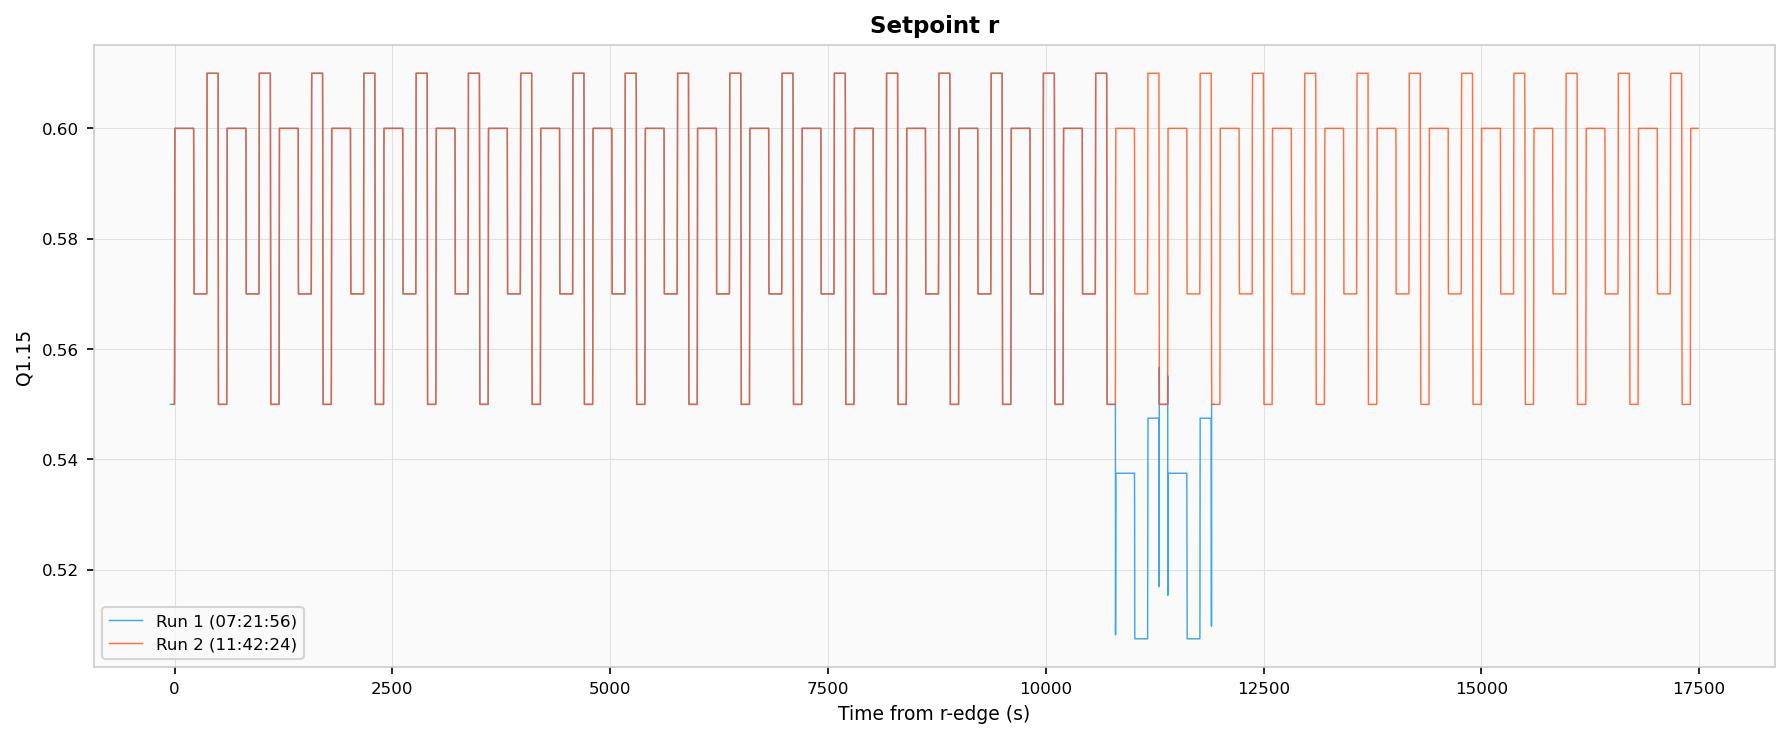
\includegraphics[width=\textwidth]{figures/ch8/01_r_overlay.jpg}
  \caption{Setpoint $r$ overlay.  Run~1 (blue) and Run~2 (red) track
           identically for the first ${\sim}10{,}000$\,s.  Run~1
           exhibits corrupted setpoint values after $t = 10{,}000$\,s,
           temporally distinct from the plant-state decay onset at
           $t \approx 2{,}500$\,s.}
  \label{fig:bench_r_overlay}
\end{figure}

% ------------------------------------------------------------
\subsection{Plant-State Decay}
\label{ssec:bench_obs_decay}
% ------------------------------------------------------------

The primary failure signature in Run~1 is a smooth, monotonic decay of
both plant-model node temperatures ($T_f$ and $T_c$), the outlet
temperature~$y$, and the measured feedback signal~$y_m$ toward zero.
The decay onset occurs at approximately $t = 2{,}500$~s and reaches the
zero clamp by approximately $t = 5{,}000$~s, a transition duration of
roughly 2\,500~s.  The decay profile is approximately exponential with
no discontinuities or step changes.  Run~2 maintains stable periodic
operation throughout the same interval.
Figures~\ref{fig:bench_Tf_overlay}--\ref{fig:bench_y_overlay} show the
overlay plots for $T_f$, $T_c$, and~$y$.

\begin{figure}[htbp]
  \centering
  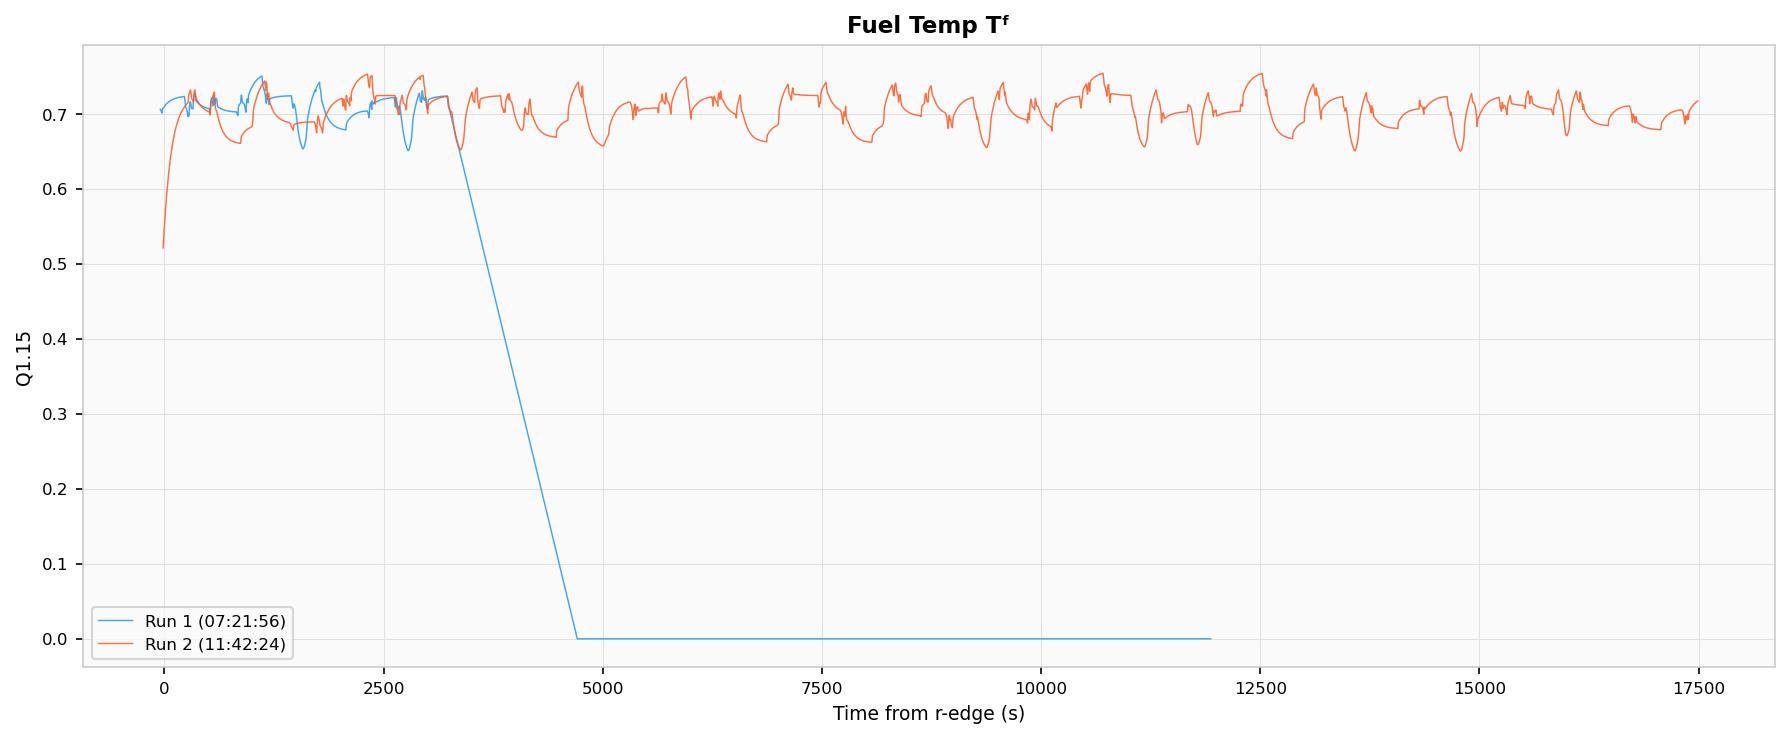
\includegraphics[width=\textwidth]{figures/ch8/08_Tf_overlay.jpg}
  \caption{Fuel temperature $T_f$ overlay.  Run~1 (blue) begins a smooth
           decay near $t = 2{,}500$\,s, reaching the zero clamp by
           $t \approx 5{,}000$\,s.  Run~2 (red) maintains stable
           periodic operation.}
  \label{fig:bench_Tf_overlay}
\end{figure}

\begin{figure}[htbp]
  \centering
  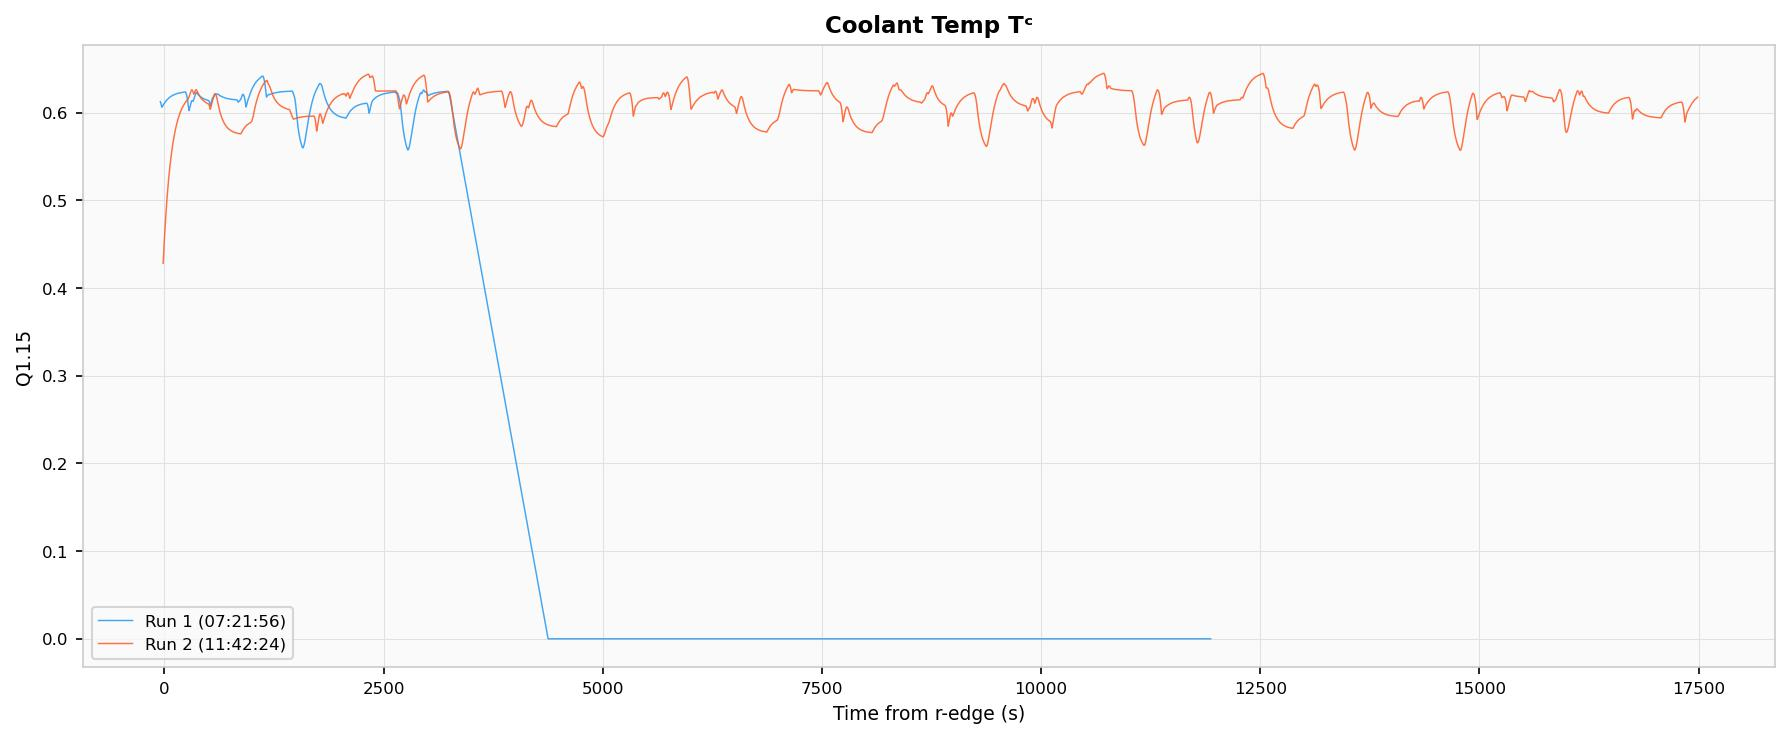
\includegraphics[width=\textwidth]{figures/ch8/09_Tc_overlay.jpg}
  \caption{Coolant temperature $T_c$ overlay.  Same decay morphology as
           $T_f$ with a slight lag, consistent with the thermal coupling
           between the two plant nodes.}
  \label{fig:bench_Tc_overlay}
\end{figure}

\begin{figure}[htbp]
  \centering
  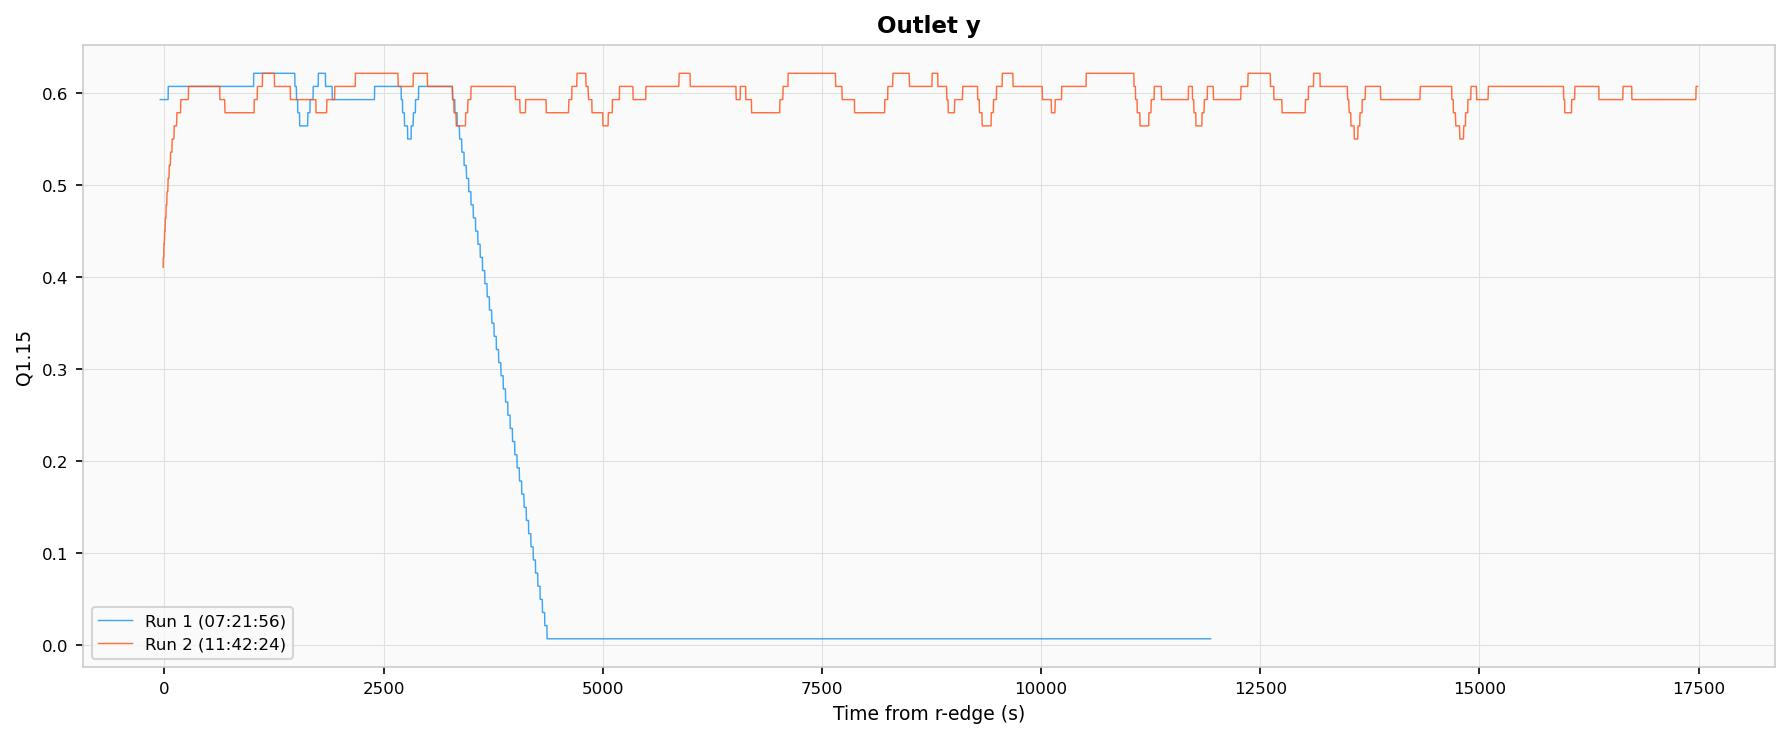
\includegraphics[width=\textwidth]{figures/ch8/04_y_overlay.jpg}
  \caption{Outlet temperature $y$ overlay.  The outlet tracks the
           coolant temperature decay through the first-order transport
           lag.}
  \label{fig:bench_y_overlay}
\end{figure}

The fuel temperature difference between runs reaches a sustained
magnitude of approximately $-0.72$ in Q1.15 units, the coolant
temperature difference reaches approximately $-0.62$, and the outlet
difference reaches approximately $-0.61$.  These are near-full-scale
departures relative to the Q1.15 representable range of $[-1,\;+1)$.
The difference traces are shown in
Figures~\ref{fig:bench_Tf_diff}--\ref{fig:bench_Tc_diff}.

\begin{figure}[htbp]
  \centering
  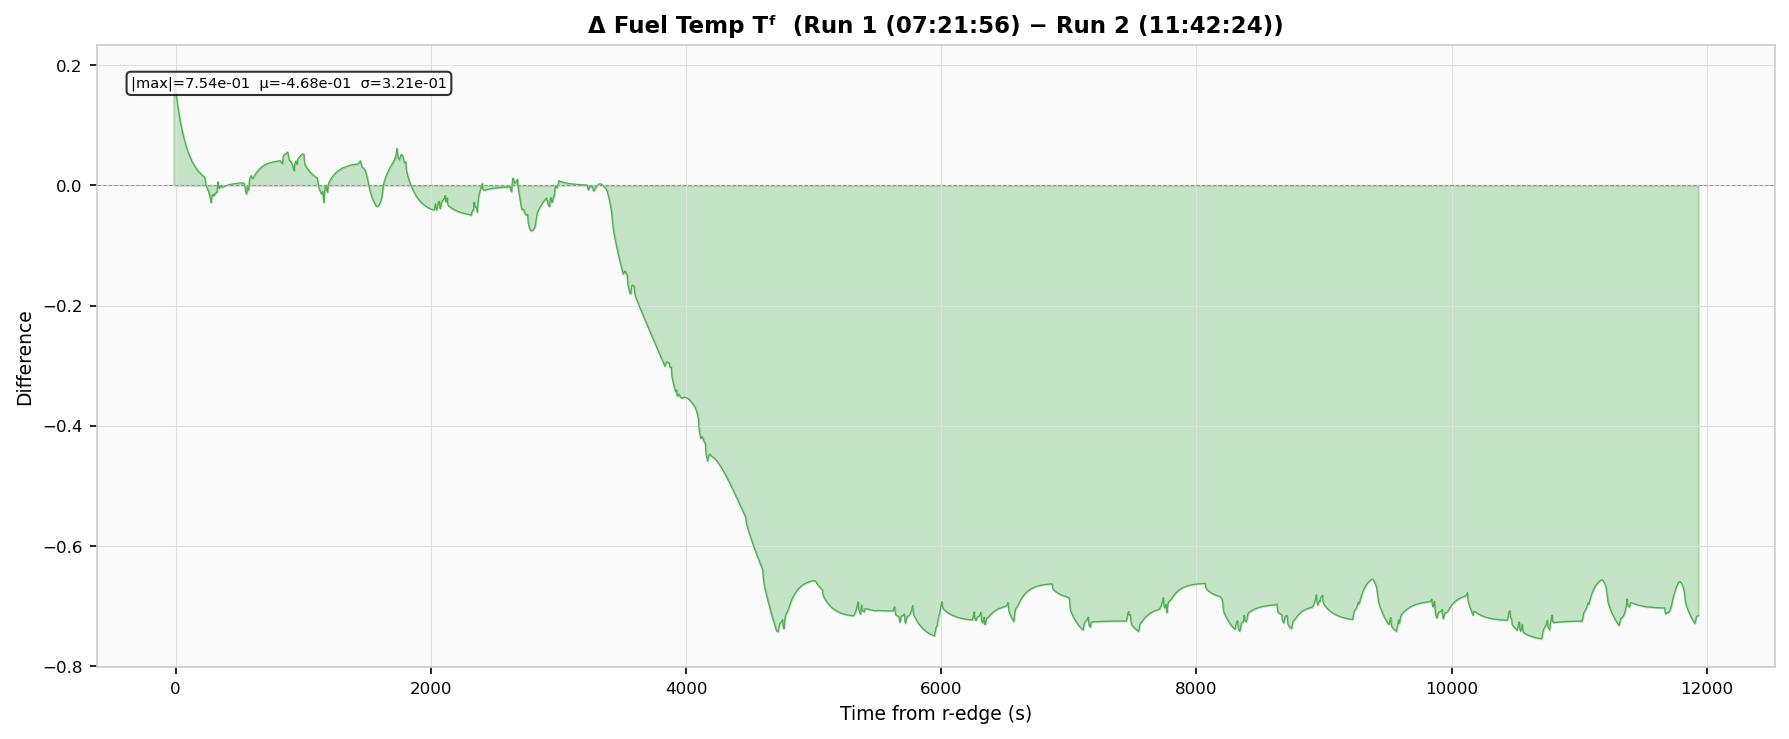
\includegraphics[width=\textwidth]{figures/ch8/18_Tf_diff.jpg}
  \caption{Fuel temperature difference (Run~1 $-$ Run~2).  The smooth
           onset near $t = 2{,}000$\,s saturates at approximately
           $-0.72$.  The difference statistics are
           $|\max| = 7.54 \times 10^{-1}$,
           $\mu = -4.68 \times 10^{-1}$,
           $\sigma = 3.21 \times 10^{-1}$.}
  \label{fig:bench_Tf_diff}
\end{figure}

\begin{figure}[htbp]
  \centering
  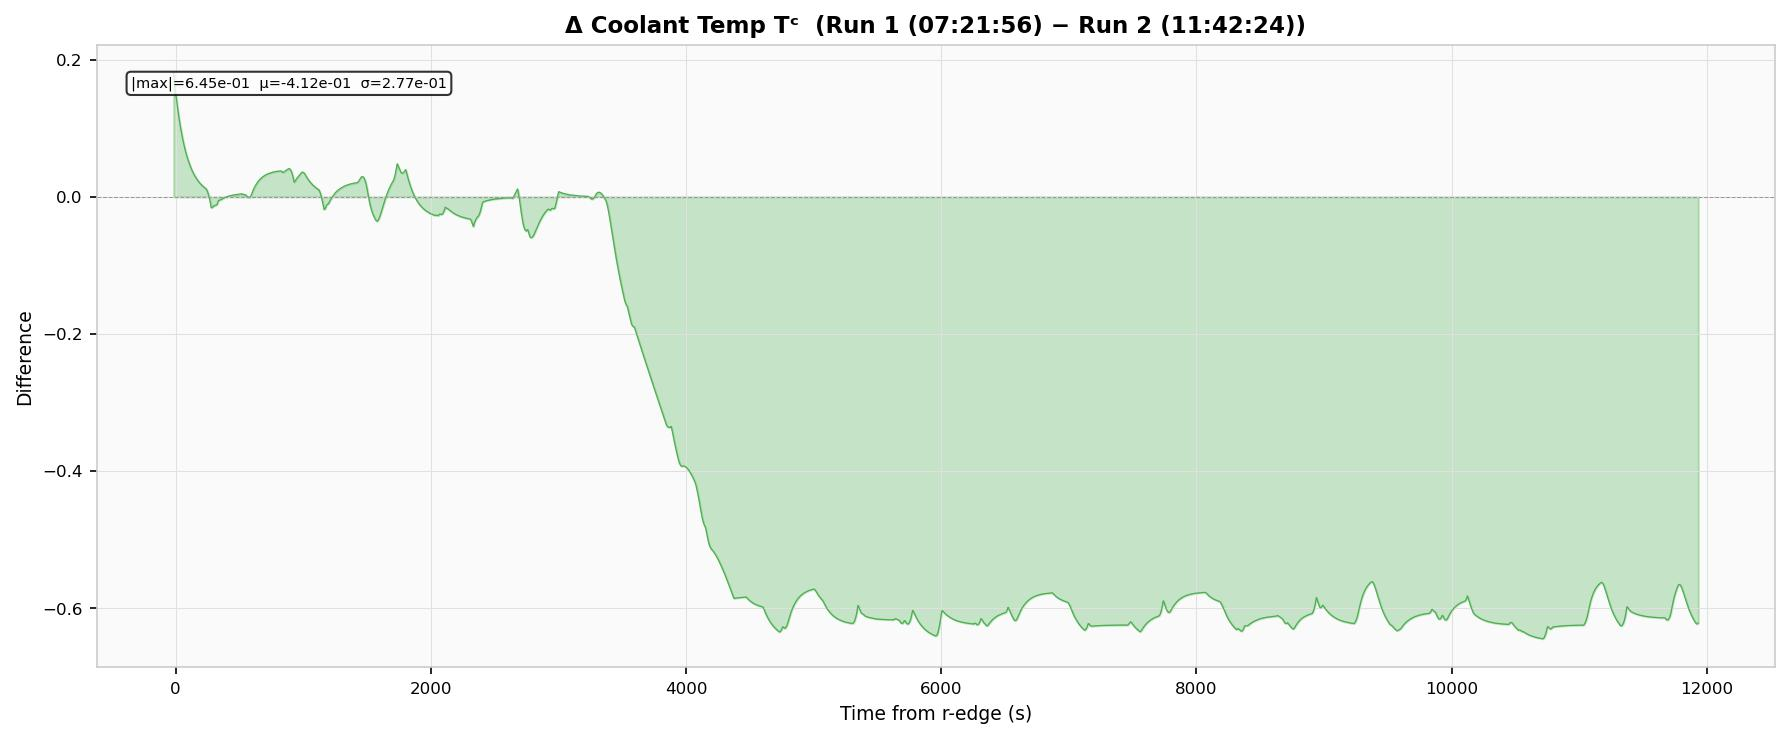
\includegraphics[width=\textwidth]{figures/ch8/19_Tc_diff.jpg}
  \caption{Coolant temperature difference (Run~1 $-$ Run~2).  Same
           morphology as the fuel temperature difference, saturating at
           approximately $-0.62$.}
  \label{fig:bench_Tc_diff}
\end{figure}

As the plant temperatures decay, the error signal ($e = r - y_m$) grows
from near-zero to approximately 0.57--0.60
(Figure~\ref{fig:bench_e_overlay}), the controller output~$u$
saturates at its limits, and the valve position~$v$ collapses to
near-zero (Figure~\ref{fig:bench_v_overlay})---all expected consequences
of the plant state approaching zero while the setpoint remains at its
nominal value.

\begin{figure}[htbp]
  \centering
  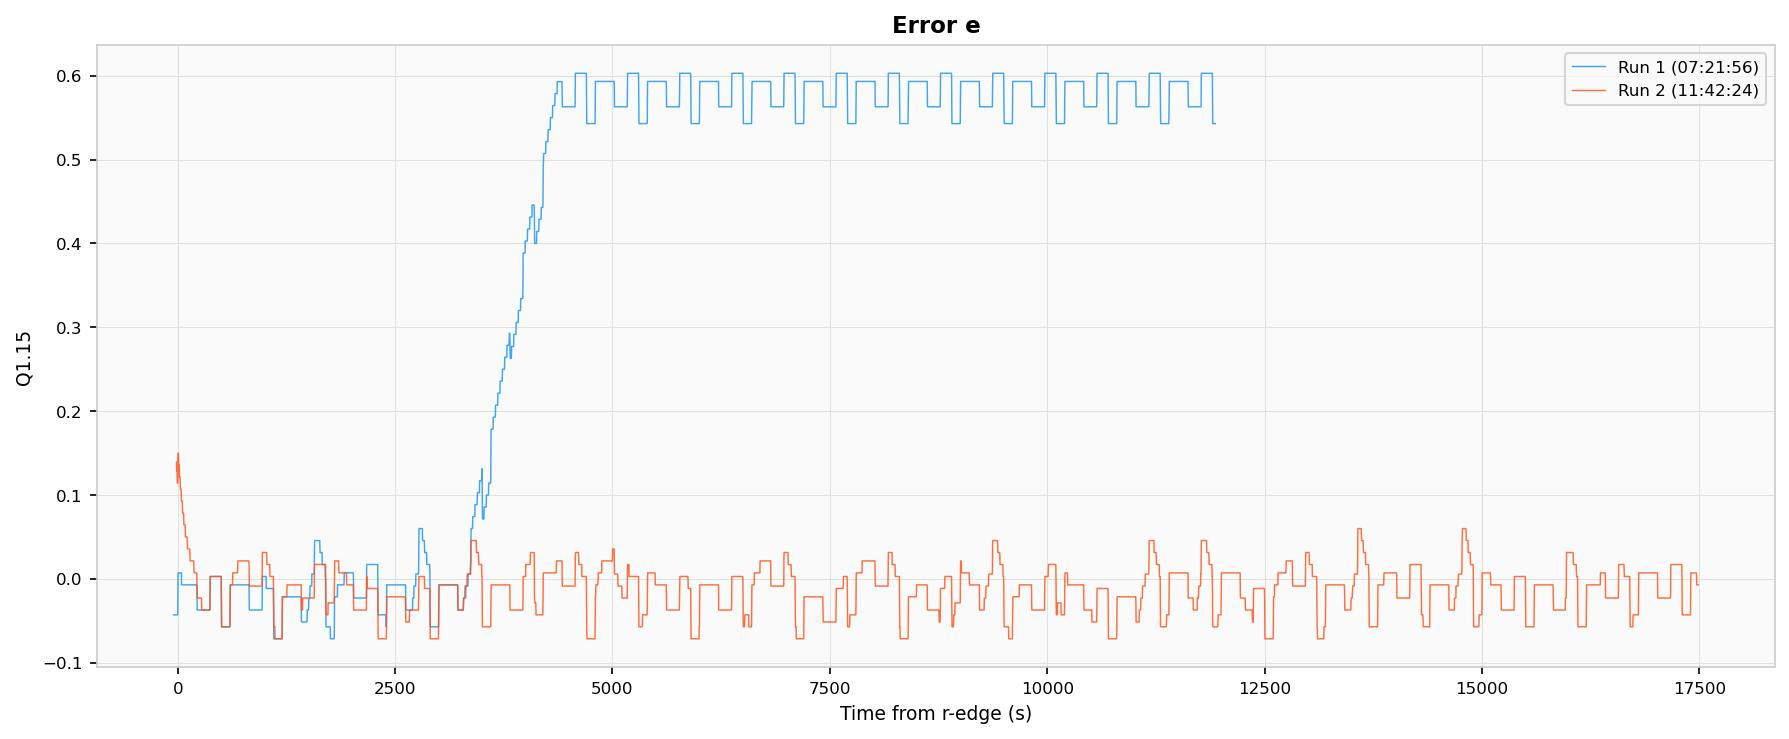
\includegraphics[width=\textwidth]{figures/ch8/10_e_overlay.jpg}
  \caption{Error signal $e = r - y_m$ overlay.  Run~1 error grows
           monotonically as plant temperatures collapse, reaching
           $e \approx 0.60$ (the setpoint value) once $y_m$ reaches
           zero.}
  \label{fig:bench_e_overlay}
\end{figure}

\begin{figure}[htbp]
  \centering
  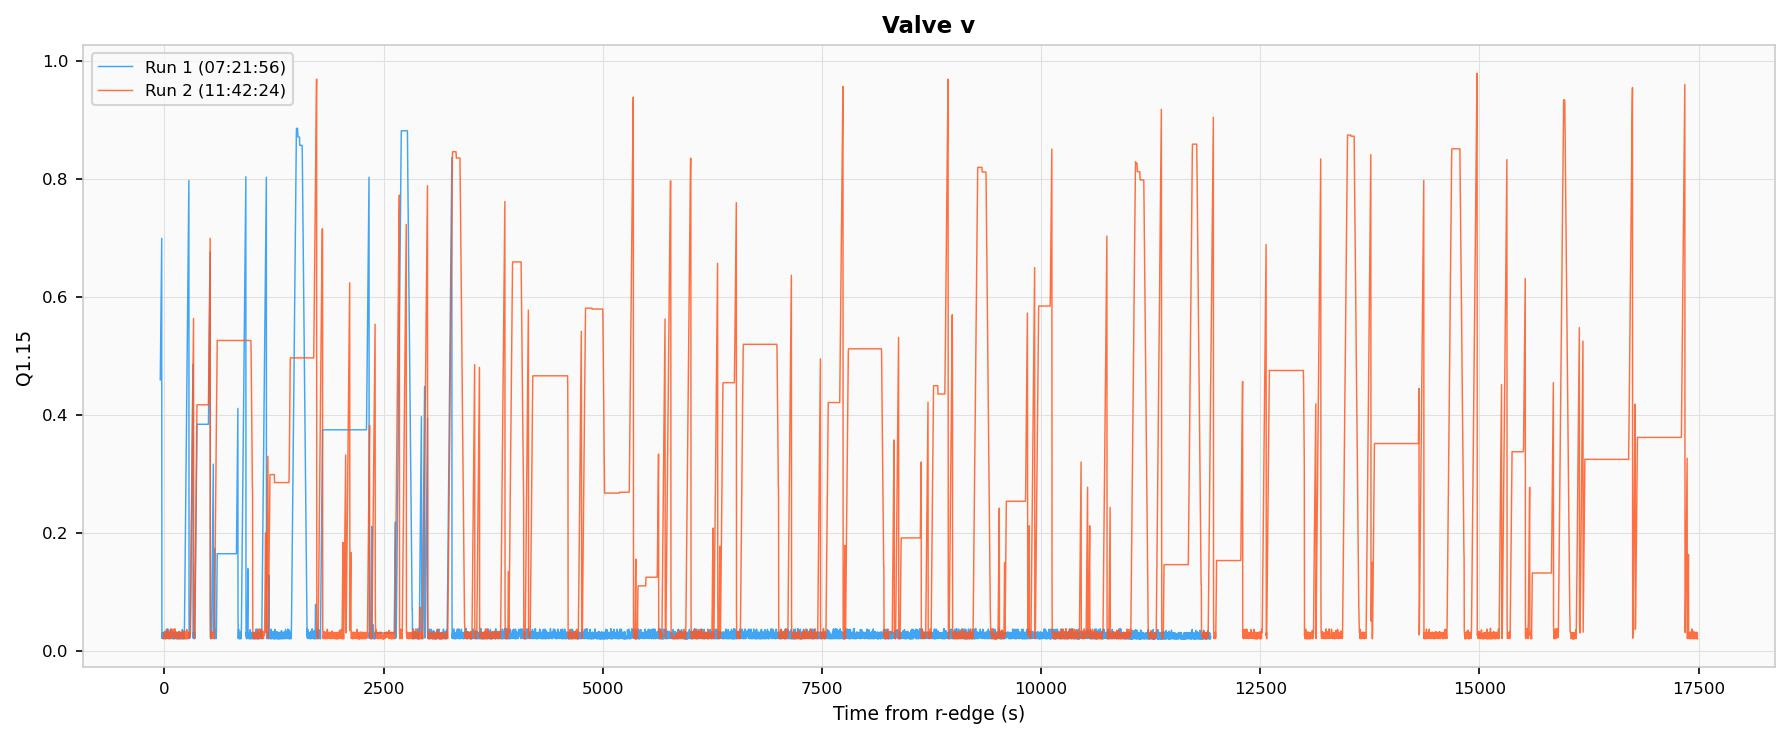
\includegraphics[width=\textwidth]{figures/ch8/07_v_overlay.jpg}
  \caption{Valve position $v$ overlay.  Run~1 (blue) valve collapses to
           near-zero after the plant-state failure.  Run~2 (red) exhibits
           the expected periodic actuation pattern driven by the ROM
           stimulus cycle.}
  \label{fig:bench_v_overlay}
\end{figure}

% ------------------------------------------------------------
\subsection{DMR Response}
\label{ssec:bench_obs_dmr}
% ------------------------------------------------------------

No DMR mismatch events were reported during the plant-state decay.  The
\texttt{dmr\_event\_count} field remained at zero throughout the entire
Run~1 acquisition.  Both redundant controller--plant chains produced
identical outputs at every compared sample tick, despite the anomalous
decay of all plant-model state variables.

% ------------------------------------------------------------
\subsection{Discussion of Failure Mechanism}
\label{ssec:bench_obs_discussion}
% ------------------------------------------------------------

\subsubsection{Exclusion of Firmware-Induced Numerical Drift}

To determine whether the observed decay could arise from numerical
accumulation effects intrinsic to the Q1.15 fixed-point arithmetic, a
bit-exact simulation of the complete closed-loop system was executed for
48~simulated hours.  The simulation reproduced the identical arithmetic
operations, rounding rules, and pipeline structure implemented in the
Verilog~RTL, including the stage-2 read-before-write dependency in the
\texttt{plant\_two\_node\_q15} module and the unsaturated integrator
update in the controller.  The simulation produced zero drift in all
state variables: the system reaches a fixed point at which every Q1.15
multiply-accumulate operation rounds to zero incremental change per tick.

Additionally, the decay morphology is inconsistent with integer overflow
or wrap-around.  An overflow of a 16-bit Q1.15 register would produce an
instantaneous polarity reversal (e.g., $+0.99$ wrapping to $-1.0$), not
a smooth 2\,500-second exponential decay.  Firmware-induced numerical
drift is therefore excluded as a causal mechanism.

\subsubsection{Exclusion of BRAM Data Corruption}

A single-event upset in a BRAM cell---for example, a corrupted entry in
the \texttt{phi\_q15} or \texttt{pow\_q15} lookup table, or a corrupted
ROM stimulus value---would affect only one of the two DMR chains, because
BRAM instances are physically separate per chain.  The resulting output
divergence would be detected by the DMR comparators.  No such detection
occurred, excluding single-chain BRAM corruption as the failure
mechanism.  This exclusion is further supported by the zero inter-run
difference observed for the shared-BRAM stimulus signals $Q$ and
$T_\mathrm{in}$.

\subsubsection{Consistency with Configuration Memory SEU}
\label{sssec:bench_cram}

The failure characteristics are collectively consistent with a
single-event upset in the FPGA configuration SRAM (CRAM).  CRAM bits
define the logic function of every lookup table (LUT), the routing of
every signal interconnect, and the configuration of every DSP48 slice.
A CRAM SEU does not alter stored data; it alters the \emph{function
computed} by the logic fabric.  Table~\ref{tab:bench_cram_evidence}
summarises the mapping between the observed failure characteristics and
the CRAM SEU mechanism.

\begin{table}[htbp]
\centering
\small
\caption{Observed failure characteristics of the PID thermal control
         benchmark and their consistency with a CRAM SEU mechanism.}
\label{tab:bench_cram_evidence}
\renewcommand{\arraystretch}{1.25}
\begin{tabular}{@{} p{4.5cm} p{8.5cm} @{}}
\toprule
\textbf{Observation} & \textbf{Consistency with CRAM SEU} \\
\midrule
DMR silent (no mismatches detected) &
CRAM bits are shared between both DMR chains.  The DMR architecture
instantiates two chains from the same synthesised netlist, placed and
routed in the same fabric.  A CRAM upset on shared parameter routing
(e.g., $K_p$, $h_{A,0}$, $T_s/C_c$) or on shared arithmetic logic
(e.g., a LUT in the coefficient builder) delivers the same corrupted
result to both chains.  The DMR comparator sees matching but incorrect
outputs. \\
\addlinespace
Smooth exponential decay (not a step or spike) &
A CRAM bit flip alters a LUT truth table for one specific input
combination, or reroutes one signal net.  This introduces a small
systematic bias in the plant integration that accumulates over many
sample ticks, producing a gradual drift rather than an instantaneous
jump. \\
\addlinespace
Temperatures decay to exactly zero (clamped) &
The \texttt{plant\_two\_node\_q15} module applies
\texttt{clamp01\_q15}, which clamps outputs to $[0,\;\texttt{0x7FFF}]$.
A negative integration bias drives temperatures through zero, where the
clamp arrests further descent. \\
\addlinespace
Onset at $t \approx 2{,}500$\,s, not at $t = 0$ &
The CRAM upset likely occurred during Day~1 irradiation (hours prior to
Run~1).  The corrupted logic path may only activate for specific input
combinations encountered during particular phases of the ROM stimulus
cycle, producing no visible effect during other phases.  The
2\,500\,s delay represents the time for the corrupted integration to
accumulate past the noise floor. \\
\addlinespace
ROM stimulus $r$ corrupts later ($t > 10{,}000$\,s) &
Consistent with a second, independent CRAM upset affecting ROM address
or data routing.  Multiple CRAM upsets are expected after hours of
cumulative irradiation. \\
\bottomrule
\end{tabular}
\end{table}

The most probable specific upset sites, given the observed decay
morphology, are:

\begin{enumerate}
\item \textbf{Routing or computation of the parameter
      \texttt{Ts\_over\_Cc}.}  This parameter has a raw Q1.15 value of~1
      (\texttt{0x0001}).  A single-bit flip to \texttt{0x0000} would
      completely disable coolant temperature integration; a flip to
      \texttt{0x8001} would invert the integration direction, causing
      $T_c$ to decay.

\item \textbf{A high-order bit in the \texttt{hA} or \texttt{mcp}
      coefficient path.}  These coefficients multiply temperature
      differences in the two-node model.  A single-bit corruption in a
      high-order bit would introduce a large systematic error in the heat
      balance, biasing the forward-Euler integration toward decay.

\item \textbf{A LUT truth-table bit in the behavioural
      \texttt{mul\_q15} function.}  The plant uses behavioural function
      calls (not the pipelined DSP48 multiplier) for its internal
      multiplies.  A corrupted LUT in this multiply chain would bias
      every product computation that traverses the affected input pattern.
\end{enumerate}

The persistence of the failure from Day~1 irradiation through the
overnight standby period and into Day~2 Run~1 is consistent with the
volatile SRAM nature of the Spartan-7 configuration store: CRAM upsets
persist until the device is reconfigured or the affected configuration
frame is scrubbed.  This mirrors the persistent UART format change
observed on FFSR1 (Chapter~\ref{chap:ffsr},
Section~\ref{subsec:ch6_disc_cfg}), and together these two independent
observations---one from a shift-register test structure, one from a
closed-loop control system---establish that configuration memory SEUs are
a primary concern for SRAM-based FPGAs at the fluence levels encountered
in this campaign.

\subsubsection{Implications for DMR Effectiveness}

The complete functional collapse of the thermal control plant with zero
DMR detection demonstrates a fundamental limitation of dual modular
redundancy when both chains share common configuration memory.  DMR
protects against BRAM data upsets (which are physically instantiated per
chain) but is transparent to CRAM logic and routing upsets (which affect
both chains identically).  Effective mitigation for this class of upset
requires either configuration memory scrubbing via ICAP/PCAP readback,
triple modular redundancy (TMR) with physical placement constraints to
ensure distinct configuration frames per voter group, or periodic
functional self-testing against known reference trajectories.

% ============================================================
\section{Relevance to Radiation-Effects Objectives}
\label{sec:bench_relevance}
% ============================================================

From a dissertation perspective, the value of this benchmark is not
only that it performs closed-loop control, but that it does so in a form
that is highly amenable to radiation-effects study.  The design
simultaneously exercises arithmetic pipelines, persistent state
registers, lookup tables, comparators, counters, and serial
communication logic---all categories of FPGA resource that can respond
differently to configuration upsets or transient single-event effects.
At the same time, the benchmark remains analytically tractable: each
module corresponds to a clear mathematical operation, and the overall
system response can be interpreted in terms of familiar control and
thermal-system theory.

The DMR wrapper transforms the benchmark from a simple controller into a
self-checking experiment.  Under nominal conditions the two chains evolve
identically, so any discrepancy is attributable to an external
perturbation.  A radiation-induced upset that perturbs logic, corrupts a
stored state, or disrupts routing within the FPGA may therefore be
detected through inter-chain divergence even if the output trajectory has
not yet become visibly unstable.  However, as the experimental results of
Section~\ref{sec:bench_observations} demonstrate, this detection
capability has an important blind spot: CRAM upsets affecting logic or
routing shared by both chains produce identical corruption in both
outputs, rendering the DMR comparator ineffective against this failure
class.  This finding refines the initial design expectation and
motivates the complementary use of configuration scrubbing or TMR with
physical separation constraints.

The combination of a meaningful closed-loop workload, bounded
fixed-point arithmetic, deterministic restart capability, and pipelined
DMR comparison makes this benchmark a well-instrumented platform that
complements the FFSR approach.  Where the FFSR experiments focused on
configuration integrity and readback verification, the fixed-point
thermal control benchmark focuses on arithmetic correctness and
control-loop functional continuity under irradiation.  Together, the two
benchmarks provide a multi-faceted evaluation of FPGA behaviour in a
neutron radiation environment relevant to nuclear instrumentation and
monitoring applications.

% ============================================================
\section{Chapter Summary}
\label{sec:bench_summary}
% ============================================================

This chapter presented the methods and algorithms used to construct the
fixed-point thermal control benchmark.  The benchmark operates as a
1\,kHz sampled-data loop on a 100\,MHz FPGA clock and integrates a
reverse-acting I-PD controller with anti-windup
(Equations~\ref{eq:error}--\ref{eq:antiwindup}), first-order actuator
dynamics with slew limiting
(Equations~\ref{eq:valve_fo}--\ref{eq:valve_slew}), a nonlinear
equal-percentage valve map implemented as a 256-entry lookup table
(Equations~\ref{eq:equal_pct}--\ref{eq:hA}), a two-node
forward-Euler thermal plant with Q1.30 internal accumulators
(Equations~\ref{eq:Tf}--\ref{eq:Tc}), an outlet transport lag
(Equation~\ref{eq:transport_lag}), a configurable quantized measurement
path (Equations~\ref{eq:quant_counts}--\ref{eq:quant_q15}), and a
dual-modular redundancy wrapper that compares six key signals on every
sample tick (Equation~\ref{eq:dmr_mismatch}).  Run gating, deterministic
restart, and 100\,Hz UART telemetry complete the design.

The neutron irradiation experiment was conducted at the OSURR fast
neutron beam facility under the same beam configuration used for the
FFSR experiments in Chapter~\ref{chap:ffsr}.  Comparative analysis of
two telemetry acquisitions---one exhibiting radiation-induced degradation
(Run~1, acquired after 19~hours of cumulative operation including Day~1
irradiation) and one serving as a nominal baseline (Run~2)---revealed a
smooth exponential decay of all plant state variables to zero over
approximately 2\,500~s, with zero DMR mismatch detection throughout.
Bit-exact 48-hour closed-loop simulation confirmed that the decay cannot
arise from firmware numerical drift.  The failure signature is consistent
with a configuration memory (CRAM) SEU affecting shared arithmetic or
routing logic, and demonstrates a fundamental limitation of DMR when both
redundant chains share common FPGA configuration memory.

By encoding the entire
benchmark in synthesizable Verilog and tying each module to explicit
mathematical relations, the design provides both a technically
meaningful control workload and a well-instrumented, self-checking
platform for the radiation-effects evaluation presented in the following
chapter.